\documentclass{article}
\usepackage[utf8]{inputenc}
\usepackage{geometry}
\usepackage{pdfpages}
\usepackage{mathtools}
\usepackage{array}
\usepackage{filecontents}
\usepackage{nicematrix}
\usepackage{bodeplot}
\graphicspath{{images/}}
\geometry{
	a4paper,
	total={170mm,257mm},
	left=20mm,
	top=20mm,
}
\usepackage{graphicx}
\usepackage{titling}
\usepackage[american,RPvoltages]{circuiTikz}
\usepackage{tikz, tikz-cd}
\usepackage{pgfplots}
\usepackage{siunitx}
\usepackage{float}
\usepackage{enumitem}
\usepackage{amsmath,amsfonts,stmaryrd,amssymb} % Math packages
\usepackage{schemabloc}
\usepackage{tcolorbox}
\usepackage{xcolor}
\usepackage[scr]{rsfso}
\newcommand*{\Scale}[2][4]{\scalebox{#1}{$#2$}}%
\newcommand*{\Resize}[2]{\resizebox{#1}{!}{$#2$}}%

\newcommand{\Laplace}{\mathscr{L}}

\title{Simulador de inductancia con OpAmp}
\author{Rodrigo}
\date{Agosto 2024}

\usepackage{fancyhdr}
\fancypagestyle{plain}{%  the preset of fancyhdr 
	\fancyhf{} % clear all header and footer fields
	\fancyfoot[L]{\thedate}
	\fancyhead[L]{Simulador de inductancia}
	\fancyhead[R]{\theauthor}
}
\makeatletter
\def\@maketitle{%
	\newpage
	\null
	\vskip 1em%
	\begin{center}%
		\let \footnote \thanks
		{\LARGE \@title \par}%
		\vskip 1em%
		%{\large \@date}%
	\end{center}%
	\par
	\vskip 1em}
\makeatother

\usepackage{lipsum}  
\usepackage{cmbright}
\renewcommand{\figurename}{Figura}
%---------------------------------------------------
\tikzset{flipflop myRS/.style={flipflop,
		flipflop def={t1=R, t3=S, t6=Q, t4={\ctikztextnot{Q}}, tu={\ctikztextnot{RST}}, nu=1, n4=1 }}
}

\tikzset{flipflop myFFRS/.style={flipflop,
		flipflop def={t1=R, t3=S, t6=Q, t4={\ctikztextnot{Q}}, n4=1 }}
}
%---------------------------------------------------

\makeatletter
\newcommand*{\underarrow}{\def\@underarrow{\relax}\@ifstar{\@@underarrow}{\def\@underarrow{\hidewidth}\@@underarrow}}
\newcommand*{\@@underarrow}[2][]{\underset{\@underarrow\substack{\uparrow\if\relax\detokenize{#1}\relax\else\\#1\fi}\@underarrow}{#2}}

\newcommand*{\overarrow}{\def\@overarrow{\relax}\@ifstar{\@@overarrow}{\def\@overarrow{\hidewidth}\@@overarrow}}
\newcommand*{\@@overarrow}[2][]{\overset{\@overarrow\substack{\if\relax\detokenize{#1}\relax\else#1\\\fi\downarrow}\@overarrow}{#2}}
\makeatother

\makeatletter
\newcounter{elimination@steps}
\newcolumntype{R}[1]{>{\raggedleft\arraybackslash$}p{#1}<{$}}
\def\elimination@num@rights{}
\def\elimination@num@variables{}
\def\elimination@col@width{}
\newenvironment{elimination}[4][0]
{
	\setcounter{elimination@steps}{0}
	\def\elimination@num@rights{#1}
	\def\elimination@num@variables{#2}
	\def\elimination@col@width{#3}
	\renewcommand{\arraystretch}{#4}
	\start@align\@ne\st@rredtrue\m@ne
}
{
	\endalign
	\ignorespacesafterend
}
\newcommand{\eliminationstep}[2]
{
	\ifnum\value{elimination@steps}>0\sim\quad\fi
	\left[
	\ifnum\elimination@num@rights>0
	\begin{array}
		{@{}*{\elimination@num@variables}{R{\elimination@col@width}}
			|@{}*{\elimination@num@rights}{R{\elimination@col@width}}}
		\else
		\begin{array}
			{@{}*{\elimination@num@variables}{R{\elimination@col@width}}}
			\fi
			#1
		\end{array}
		\right]
		& 
		\begin{array}{l}
			#2
		\end{array}
		&%                                    moved second & here
		\addtocounter{elimination@steps}{1}
	}
	\makeatother
	
	\makeatletter
	\renewcommand*\env@matrix[1][*\c@MaxMatrixCols c]{%
		\hskip -\arraycolsep
		\let\@ifnextchar\new@ifnextchar
		\array{#1}}
	\makeatother
	
\setlength\parindent{0pt}
\begin{document}
	
	\maketitle
	
	\noindent\begin{tabular}{@{}ll}
		Author & \theauthor\\

	\end{tabular}

	
	\section*{Análisis}
El método más directo para transformar un filtro pasivo en un circuito activo sin inductores es reemplazar todos sus inductores por circuitos activos con comportamiento inductivo, estos son referidos como inductores simulados. Los inductores simulados son circuitos de un puerto en el cual la impedancia de entrada es de la for,a $Z_{in}(s) = sL$. A pesar de que hay muchos circuitos que se comportan como inductores, los más populares son los circuitos de Riordan y de Antoniou, los cuales han sido usados por varias décadas.

\section{Indcutor simulado de Riordan}

	
	\begin{figure}[H]
		\centering	
		\begin{tikzpicture}[scale=0.8]
			\ctikzset{resistor = european}
			\ctikzset{bipoles/thickness=4}
			\ctikzset{monopoles/vcc/arrow={Stealth[width=6pt,length=9pt]}}
			\ctikzset{monopoles/vee/arrow={Stealth[width=6pt,length=9pt]}}
			\draw (0,0) node[op amp, noinv input up, anchor=+](OA1){$OA_1$};
			\draw (OA1.-) to[short] ++(-1,0)
			      to[short] ++(0,-2) coordinate (p1);
			\draw (p1) to[R, l=$Z_2$] (p1 -| OA1.out) to[short] (OA1.out) node[above]{$V_1$};
			\draw (p1) to[R, *-, l=$Z_1$] ++(0,-4) coordinate (z1) node[ground]{};
			\draw (OA1.out) to[R, *-*, l=$Z_3$] ++(4,0) node[above]{$V_n$} coordinate (p2);
			\draw (p2) to[short] ++(1,0) coordinate (p3);
			\draw (p3) node[op amp, noinv input up, anchor=-](OA2){$OA_2$};
			\draw (p2) to[short] ++(0,-2) coordinate (p4);
			\draw (p4) to[R, l=$Z_4$] (p4 -| OA2.out) to[short] (OA2.out);
			\draw (OA2.+) to[short] ++(-1,0)
			      to[short] ++(0,2) coordinate (p5);
			\draw (p5) to[R, l=$Z_5$] (p5 -| OA2.out) to[short, -*] (OA2.out) node[right]{$V_2$};		
			\draw (OA1.+) to[short] ++(-1,0) coordinate (p6) to[short] (p1|-p5) to[short, -*] (p5);
			\draw (p6) to[short, *-o, f_<=$I(s)$] ++(-2,0) coordinate (z2) node[left]{$E(s)$};
			\draw (z1) to[short, *-o] ++(-2,0);
			\coordinate (M) at ($(z2)!0.5!(z1)$);
			\draw[->]  (M)++(-1,0) node[left]{$Z_{in}(s)$} -- ++(1,0);
 		\end{tikzpicture}
		\caption{Inductor simulado de Riordan}	
		\label{fig:figura1}
	\end{figure}
	
Podemos reconocer que el amplificador $OA_1$ se trata de un amplificador no inversor, por lo tanto, el voltaje en el nodo $V_1$ es:

\begin{align}
	V_1(s) = \frac{Z_1(s) + Z_2(s)}{Z_1(s)}E(s)
\end{align}

La aplicación de la LCK en la terminal no inversora del amplificador $OA_2$ produce

\begin{align}
	I(s) = I_{z_5}(s)
\end{align}

O bien

\begin{align}
	I(s) = \frac{E(s) - V_2(s)}{Z_5(s)}
\end{align}

Ahora aplicamos la LCK en el nodo $V_n$

\begin{align}
	I_{z_3}(s) = I_{z_4}(s)
\end{align}

Mediante ley Ohm, representamos (4) como

\begin{align}
	\frac{V_1(s) - V_n(s)}{Z_3(s)} = \frac{V_n(s) - V_2(s)}{Z_4(s)}
\end{align}

Sin embargo

\begin{align}
	V_n(s) = E(s)
\end{align}

La sustitución de la ecuación (6) en (5) produce

\begin{align}
	\frac{V_1(s) - E(s)}{Z_3(s)} = \frac{E(s) - V_2(s)}{Z_4(s)}
\end{align} 

Despejamos $V_2(s)$ de la ecuación (7)

\begin{align}
	Z_4(s)V_1(s) &- Z_4(s)E(s) = Z_3(s)E(s) - Z_3(s)V_2(s) \nonumber \\
	Z_4(s)V_1(s) &- Z_4(s)E(s) - Z_3(s)E(s) = - Z_3(s)V_2(s) \nonumber \\
	V_2(s) &= \frac{Z_3(s) + Z_4(s)}{Z_3(s)}E(s) - \frac{Z_4(s)}{Z_3(s)}V_1(s)
\end{align} 

Sustituimos (1) en (8)
\begin{align}
	V_2(s) &= \frac{Z_3(s) + Z_4(s)}{Z_3(s)}E(s) - \frac{Z_4(s)}{Z_3(s)} \left[ \frac{Z_1(s) + Z_2(s)}{Z_1(s)} \right] E(s)
\end{align}

Por último, sustituimos (9) en (3)

\begin{align}
	I(s) &= \frac{E(s) - \frac{Z_3(s) + Z_4(s)}{Z_3(s)}E(s) - \frac{Z_4(s)}{Z_3(s)} \left[ \frac{Z_1(s) + Z_2(s)}{Z_1(s)} \right] E(s) }{Z_5(s)} \nonumber \\
	&= \frac{ \left[ 1 - \frac{Z_3(s) + Z_4(s)}{Z_3(s)} - \frac{Z_4(s)}{Z_3(s)} \left[ \frac{Z_1(s) + Z_2(s)}{Z_1(s)}  \right] \right]E(s) }{Z_5(s)} \nonumber \\
	&= \frac{ \left[ \frac{ Z_1(s)Z_3(s) - Z_1(s)(Z_3(s) + Z_4(s)) - Z_4(s)(Z_1(s) + Z_2(s)) }{ Z_1(s) Z_3(s) } \right] E(s) }{Z_5(s)} \nonumber \\
	&= \frac{ \left[ \frac{ Z_1(s)Z_3(s) - Z_1(s)Z_3(s) - Z_1(s)Z_4(s) - Z_1(s)Z_4(s) + Z_2(s)Z_4(s) }{ Z_1(s) Z_3(s) } \right] E(s) }{Z_5(s)} \nonumber \\
	&= \frac{ \frac{Z_2(s)Z_4(s)}{Z_1(s)Z_3(s)} }{Z_5(s)} E(s) \nonumber
\end{align}

Es decir

\begin{align}
	I(s) = \frac{Z_2(s)Z_4(s)}{Z_1(s)Z_3(s)Z_5(s)}E(s)
\end{align}

Así, la impedancia $Z_{IN}(s)$ está dada por
\begin{align}
	Z_{IN}(s) = \frac{E(s)}{I(s)} = \frac{Z_2(s)Z_4(s)}{Z_1(s)Z_3(s)Z_5(s)}
\end{align}

Es claro ver que si $Z_2(s)$ es un capacitor con impedancia $Z_2(s) = \frac{1}{sC_2}$ y las demás impedancias $Z_i(S)$ son resistores $R_i$ como en la figura 2, la impedancia de entrada se vuelve

\begin{align}
	Z_{IN}(s) = s\frac{R_1R_3R_5C_2}{R_4}
\end{align}

	\begin{figure}[H]
	\centering	
	\begin{tikzpicture}[scale=0.8]
		%\ctikzset{resistor = european}
		\ctikzset{bipoles/thickness=4}
		\ctikzset{monopoles/vcc/arrow={Stealth[width=6pt,length=9pt]}}
		\ctikzset{monopoles/vee/arrow={Stealth[width=6pt,length=9pt]}}
		\draw (0,0) node[op amp, noinv input up, anchor=+](OA1){$OA_1$};
		\draw (OA1.-) to[short] ++(-1,0)
		to[short] ++(0,-2) coordinate (p1);
		\draw (p1) to[C, l=$C_2$] (p1 -| OA1.out) to[short] (OA1.out) node[above]{$V_1$};
		\draw (p1) to[R, *-, l=$R_1$] ++(0,-4) coordinate (z1) node[ground]{};
		\draw (OA1.out) to[R, *-*, l=$R_3$] ++(4,0) node[above]{$V_n$} coordinate (p2);
		\draw (p2) to[short] ++(1,0) coordinate (p3);
		\draw (p3) node[op amp, noinv input up, anchor=-](OA2){$OA_2$};
		\draw (p2) to[short] ++(0,-2) coordinate (p4);
		\draw (p4) to[R, l=$R_4$] (p4 -| OA2.out) to[short] (OA2.out);
		\draw (OA2.+) to[short] ++(-1,0)
		to[short] ++(0,2) coordinate (p5);
		\draw (p5) to[R, l=$R_5$] (p5 -| OA2.out) to[short, -*] (OA2.out) coordinate (np) node[right]{$V_2$};		
		\draw (OA1.+) to[short] ++(-1,0) coordinate (p6) to[short] (p1|-p5) to[short, -*] (p5);
		\draw (p6) to[short, *-o, f_<=$I(s)$] ++(-2,0) coordinate (z2) node[left]{$E(s)$};
		\draw (z1) to[short, *-o] ++(-2,0);
		\coordinate (M) at ($(z2)!0.5!(z1)$);
		\draw[->]  (M)++(-1,0) node[left]{$Z_{in}(s)$} -- ++(1,0);
		
		\draw (np)++(2,0) to[short, o-] ++(2,0)
		      to[L, -*, l={$L = \frac{R_1R_3R_5C_2}{R_4}$}] ++(0,-4) coordinate (l1)
		      to[short, -o] ++(-2,0);
		\draw (l1) node[ground]{};
	\end{tikzpicture}
	\caption{Inductor simulado de Riordan sustituyendo las impedancias por sus elementos resistivos y capacitivo}	
	\label{fig:figura2}
\end{figure}

El cual representa un inductor cuya inductancia está dada por

\begin{align}
	L = \frac{R_1R_3R_5C_2}{R_4}
\end{align}

Dado que una de las terminales del puerto de entrada del circuito de Riordan está puesta a tierra, este circuito sólo puede simular inductores puestos a tierra. Finalmente, debemos notar que si $Z_4(s)$ es un capacitor con una impedancia $Z_4(s) = \frac{1}{sC_4}$ y las demás impedancias $Z_i(s)$ son resistores $R_i$, el circuito simularía un inductor con un valor de

\begin{align}
	L = \frac{R_1R_3R_5C_4}{R_2}
\end{align}

\subsection{Ejemplo 1}
El circuito de la figura 3 muestra un filtro pasivo pasa altas Chebyshev de orden $N = 3$, diseñado para satisfacer las siguientes condiciones:

\begin{align}
	f_c = \qty{10}{\kilo \hertz} \quad f_s = \qty{333.33}{\kilo \hertz} \quad A_{max} = \qty{0.5}{\decibel} \quad A_{min} = \qty{20}{\decibel} \nonumber
\end{align}

Diseñe un circuito de Riordan de manera que simule el comportamiento del inductor en el filtro.

	\begin{figure}[H]
	\centering	
	\begin{tikzpicture}[scale=0.8]
		%\ctikzset{resistor = european}
		\ctikzset{bipoles/thickness=4}
		\ctikzset{monopoles/vcc/arrow={Stealth[width=6pt,length=9pt]}}
		\ctikzset{monopoles/vee/arrow={Stealth[width=6pt,length=9pt]}}
		\draw (0,0)++(5,0) coordinate (origin) to[R, o-, l=$R_6$, a_=$\qty{1}{\kilo \ohm}$] ++(3,0)
		      to[C, l=$C_1$, a_=$\qty{9.98}{\nano \farad}$] ++(3,0) coordinate (p1)
		      to[C, *-, l=$C_3$, a_=$\qty{9.98}{\nano \farad}$] ++(6,0)
		      to[R, l2=$R_L$ and $\qty{1}{\kilo \ohm}$] ++(0,-4) coordinate (p2);
		\draw (p1) to[L, -*, l2=$L_1$ and $\qty{14.52}{\milli \henry}$] ++(0,-4) node[ground]{}; 
		\draw (p2) to[short, -o] (p2 -| origin) coordinate (p3);
		\draw (origin) to[open, v=$E(s)$] (p3);
	\end{tikzpicture}
	%\caption{Filtro pasa altas de tercer orden con un inductor simulado de Riordan}	
	%\label{fig:figura3}
\end{figure}

	\begin{figure}[H]
	\centering	
	\begin{tikzpicture}[scale=0.8]
		%\ctikzset{resistor = european}
		\ctikzset{bipoles/thickness=4}
		\ctikzset{monopoles/vcc/arrow={Stealth[width=6pt,length=9pt]}}
		\ctikzset{monopoles/vee/arrow={Stealth[width=6pt,length=9pt]}}
		\draw (0,0) node[op amp, noinv input up, anchor=+](OA1){$OA_1$};
		\draw (OA1.-) to[short] ++(-1,0)
		to[short] ++(0,-2) coordinate (p1);
		\draw (p1) to[R, l=$C_2$] (p1 -| OA1.out) to[short] (OA1.out);
		\draw (p1) to[R, *-, l=$R_1$] ++(0,-4) coordinate (z1) node[ground]{};
		\draw (OA1.out) to[R, *-*, l=$R_3$] ++(4,0) coordinate (p2);
		\draw (p2) to[short] ++(1,0) coordinate (p3);
		\draw (p3) node[op amp, noinv input up, anchor=-](OA2){$OA_2$};
		\draw (p2) to[short] ++(0,-2) coordinate (p4);
		\draw (p4) to[R, l=$R_4$] (p4 -| OA2.out) to[short] (OA2.out);
		\draw (OA2.+) to[short] ++(-1,0)
		to[short] ++(0,2) coordinate (p5);
		\draw (p5) to[R, l=$R_5$] (p5 -| OA2.out) to[short, -*] (OA2.out);		
		\draw (OA1.+) to[short] ++(-1,0) coordinate (p6) to[short] (p1|-p5) coordinate (c1) to[short, -*] (p5);
		\draw (c1) to[short, *-*] ++(0,3) coordinate (c2)
		      to[C, l_=$C_1$, a^=$\qty{9.98}{\nano \farad}$] ++(-3,0)
		      to[R, -o, l_=$R_6$, a^= $\qty{1}{\kilo\ohm}$] ++(-3,0) coordinate(c4);
		 \draw (c2) to[C, l^=$C_3$, a=$\qty{9.98}{\nano \farad}$] ++(15,0) coordinate (c3);
		 \draw (c3) to[R, l2=$R_L$ and $\qty{1}{\kilo \ohm}$] (c3 |- z1) to[short, -*] (z1) to [short, -o] ++(-6,0) coordinate (c5);
		 \draw (c4) to[open, v=$E(s)$] (c4 |- c5);
	\end{tikzpicture}
	\caption{Filtro pasa altas de tercer orden con un inductor simulado de Riordan}	
	\label{fig:figura4}
\end{figure}

El inductor puesto a tierra en el filtro pasivo es reemplazado por su circuito equivalente de Riordan. Si hacemos que $R_3 = R_4 = R_5 = R$ y $C = \qty{9.98}{\nano \farad}$, entonces el valor de $R_1$ puede calcularse de $R_1 = \frac{L_2}{RC_2}$. Para $R = \qty{1}{\kilo \ohm}, C_2 = \qty{9.98}{\nano \farad}$ y $L_2 = \qty{14.52}{\milli \henry}$ obtenemos $R_1 = \qty{1.455}{\kilo \ohm}$. La gráfica de Bode tanto del circuito activo como del circuito pasivo son idénticas, como se muestra en la figura 5.

\begin{figure}[H]
	\centering
	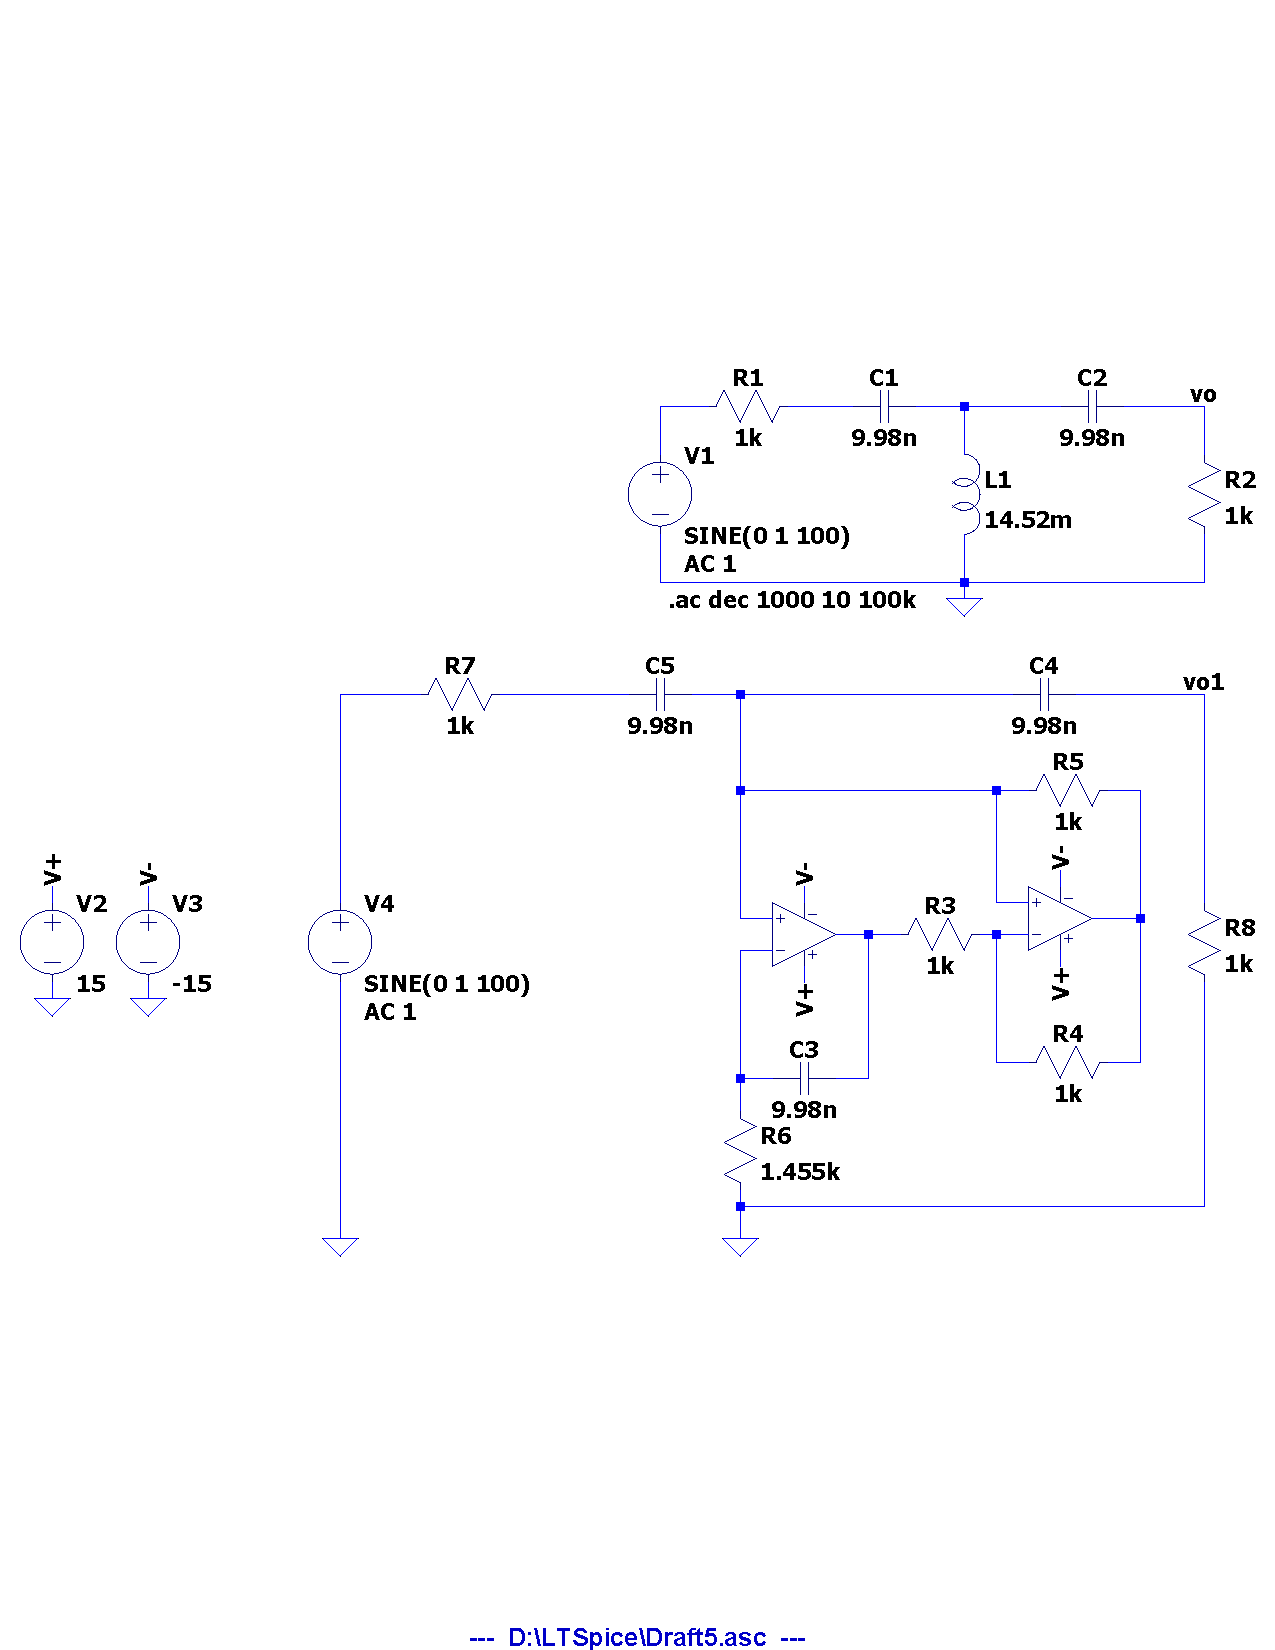
\includegraphics[clip, trim=0cm 6.5cm 0cm 6cm, width=\textwidth]{bodePlotCircuit}
	\caption{Circuito esquemático}	
	\label{fig:figura5}
\end{figure}

\begin{figure}[H]
	\centering
	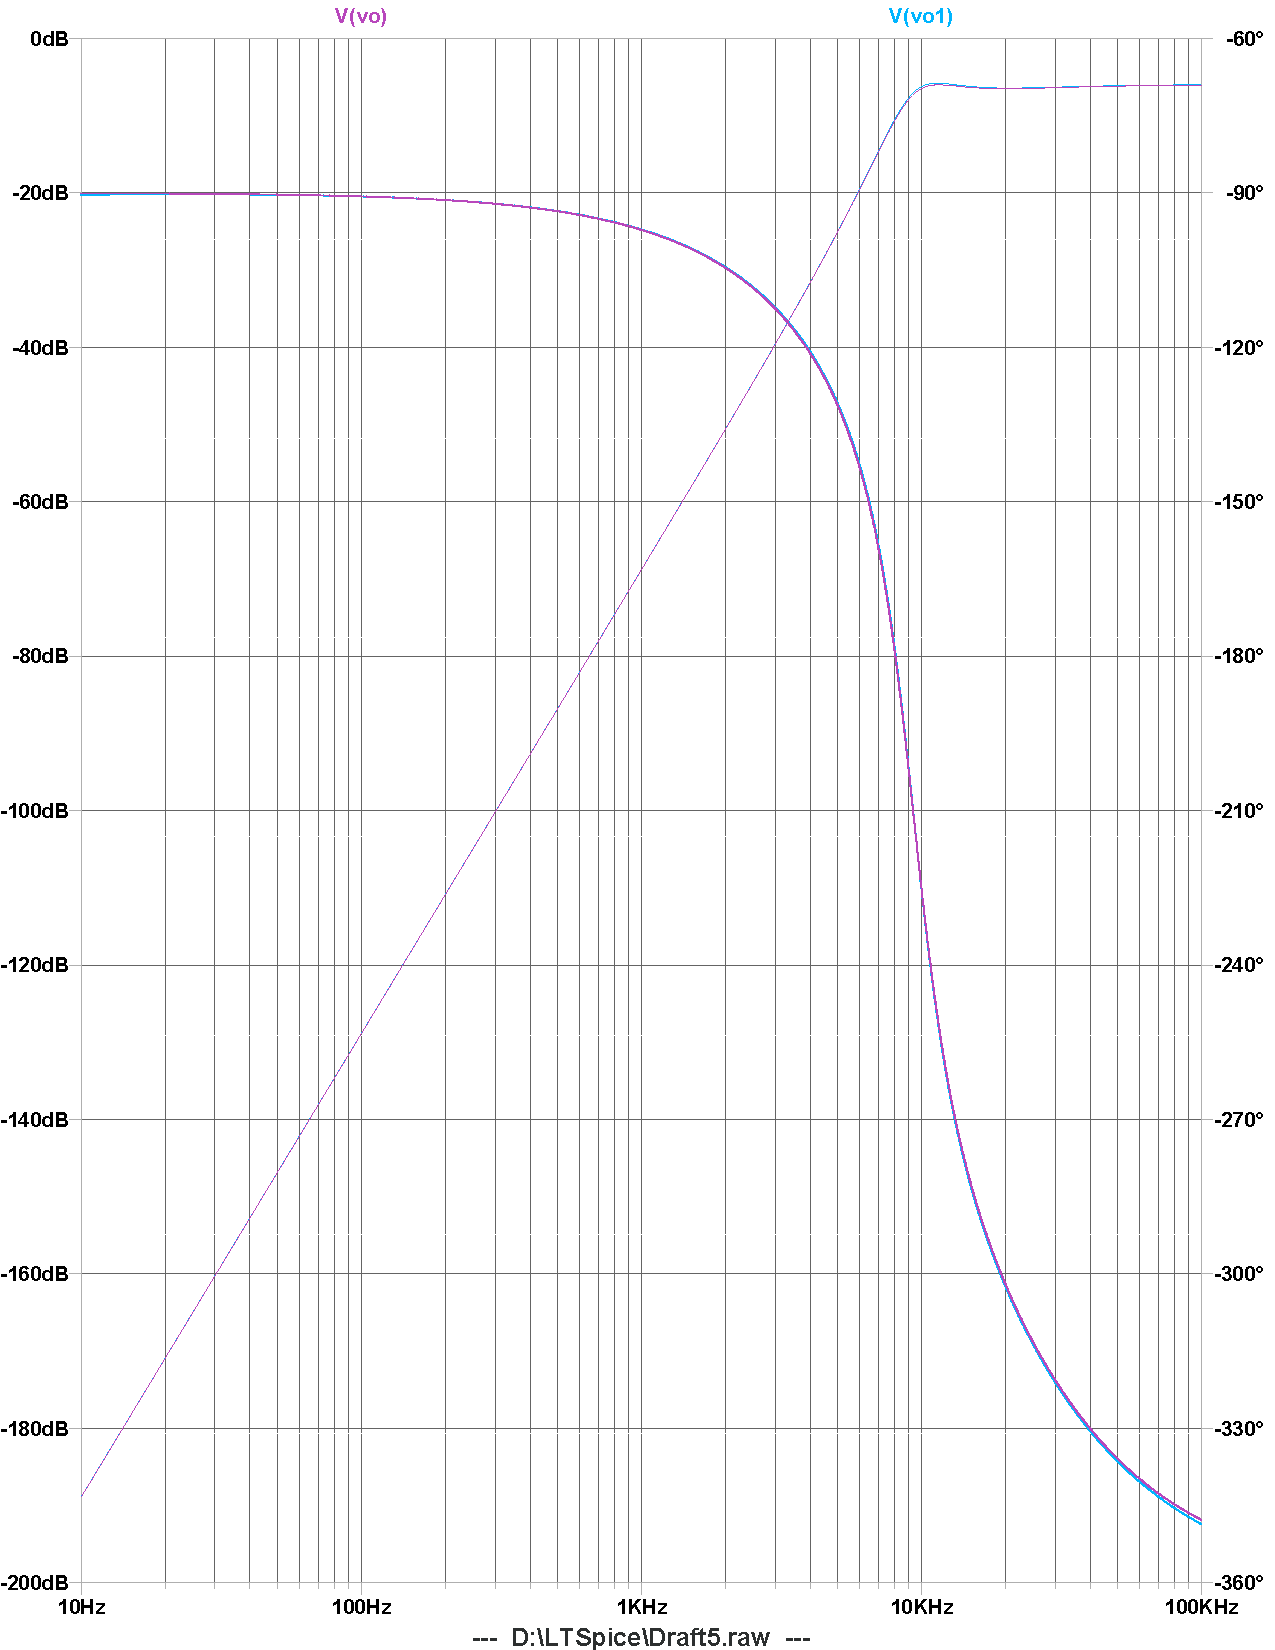
\includegraphics[clip, trim=0cm 0.5cm 0cm 0cm, width=\textwidth]{bodeplot}
	\caption{Gráfica de $v_o$ vs $v_{o_1}$}	
	\label{fig:figura6}
\end{figure}

\newpage
\section{Inductor sumulado de Antoniou}

	\begin{figure}[H]
	\centering	
	\begin{tikzpicture}[scale=0.8]
		\ctikzset{resistor = european}
		\ctikzset{bipoles/thickness=4}
		\ctikzset{monopoles/vcc/arrow={Stealth[width=6pt,length=9pt]}}
		\ctikzset{monopoles/vee/arrow={Stealth[width=6pt,length=9pt]}}
		\draw (0,0) node[op amp, noinv input up, anchor=+, rotate=90](OA1){$OA_1$};
		\draw (OA1.+) to[short] ++(-3,0)
		      to[short] ++(0,-1.5) coordinate (p1);
		\draw (OA1.-) to[short] ++(3,0)
		      to[short] ++(0,-1.5) coordinate (p2) node[above right]{$V_x$};
		\coordinate (M) at ($(p1)!0.5!(p2)$) ;
		\draw (p1) to[R, -*, f>^=$I(s)$, l=$Z_1$] (M) node[above]{$V_2$}
		      to[R, l=$Z_2$, -*] (p2);
		\draw (p2) to[short] ++(0,-1.5)
		      to[short] ++(3,0) coordinate(p3);
		\draw (p3) node[op amp, anchor=-, rotate=-90, noinv input up](OA2){$OA_2$};
		\draw (OA2.+) to[short] ++(3,0)
		      to[short] ++(0,1.5) coordinate (p4);  
	    \coordinate (M1) at ($(p2)!0.5!(p4)$);
	    \draw (p2) to[R, l=$Z_3$, -*] (M1);
	    \draw (M1) to[R, l=$Z_4$, -*,] (p4);
	    \draw (OA1.out) to[short] (OA1.out) -| (M1) node[above right]{$V_1$};
	    \draw (OA2.out) to[short] (OA2.out) -| (M);
	    \draw (p4) to[R, l=$Z_5$] ++(3,0)
	          to[short, -*] ++(0,-5.5) coordinate (o2) node[ground]{};
	    \draw (p1) to[short, *-o, f_<=$I(s)$] ++(-2,0) coordinate (o1) node[left]{$E(s)$};
	    \draw (o2) to[short, -o] (o2 -| o1) coordinate (o3);
	    \coordinate (M2) at ($(o1)!0.5!(o3)$);
	    \draw[->]  (M2)++(-1,0) node[left]{$Z_{in}(s)$} -- ++(1,0);
	\end{tikzpicture}
	\caption{Inductor simulado de Antoniou}	
	\label{fig:figura7}
\end{figure}

Empleando la LCK en el nodo $V_y$ obtenemos
\begin{align}
	I_{z_4}(s) = I_{z_5}(s)
\end{align}

Mediante ley de Ohm:

\begin{align}
	\frac{V_1(s) - V_y(s)}{Z_4(s)} = \frac{V_y(s)}{Z_5(s)}
\end{align}

Sin embargo, tenemos que $V_y(s) = V_x(s) = E(s)$, por lo tanto
\begin{align}
	\frac{V_1(s) - E(s)}{Z_4(s)} = \frac{E(s)}{Z_5(s)} \nonumber \\
	Z_5(s)V_1(s) - Z_5(s)E(s) = Z_4(s)E(s) \nonumber \\
	V_1(s) = \frac{Z_4(s) + Z_5(s)}{Z_5(s)}E(s)
\end{align}

Ahora empleamos la LCK en el nodo $V_x$
\begin{align}
	I_{z_2}(s) = I_{z_3}(s)
\end{align}

O bien

\begin{align}
	\frac{V_2(s) - E(s)}{Z_2(s)} &= \frac{E(s) - V_1(s)}{Z_3(s)} \nonumber \\
	Z_3(s)V_2(s) - Z_3(s)E(s) &= Z_2(s)E(s) - Z_2(s)V_1(s)
\end{align}

Despejamos $V_2(s)$ de la ecuación (19)

\begin{align}
	V_2(s) = \frac{Z_2(s) + Z_3(s)}{Z_3(s)}E(s) - \frac{Z_2(s)}{Z_3(s)}V_1(s)
\end{align}

Sustituimos (17) en (20)

\begin{align}
	V_2(s) &= \frac{Z_2(s) + Z_3(s)}{Z_3(s)}E(s) - \frac{Z_2(s)}{Z_3(s)} \frac{Z_4(s) + Z_5(s)}{Z_5(s)}E(s) \nonumber \\
	V_2(s) &= \frac{Z_2(s)Z_5(s) + Z_3(s)Z_5(s) - Z_2(s)Z_4(s) - Z_2(s)Z_5(s) }{Z_3(s)Z_5(s)}E(s) \nonumber \\
	V_2(s) &= \frac{Z_3(s)Z_5(s) - Z_2(s)Z_4(s)}{Z_3(s)Z_5(s)}E(s)
\end{align}

Sin embargo, tenemos que

\begin{align}
	I(s) = \frac{E(s) - V_2(s)}{Z_1(s)}
\end{align}

Sustituimos (21) en (22)
\begin{align}
	I(s) &= \frac{ \left[ 1 - \frac{Z_3(s)Z_5(s) - Z_2(s)Z_4(s)}{Z_3(s)Z_5(s)} \right]E(s) }{Z_1(s)} \nonumber \\
	I(s) &= \frac{\frac{Z_3(s)Z_5(s) - Z_3(s)Z_5(s) + Z_2(s)Z_4(s)}{Z_3(s)Z_5(s)}E(s) }{Z_1(s)} \nonumber \\
	I(s) &= \frac{ \frac{Z_2(s)Z_4(s)}{Z_3(s)Z_5(s)} }{Z_1(s)}E(s)
\end{align}

Es decir:

\begin{align}
	I(s) = \frac{Z_2(s)Z_4(s)}{Z_1(s)Z_3(s)Z_5(s)}E(s)
\end{align}

La impedancia está dada por

\begin{align}
	Z_{in}(s) = \frac{E(s)}{I(s)} = \frac{Z_1(s)Z_3(s)Z_5(s)}{Z_2(s)Z_4(s)}
\end{align}

El circuito es un convertidor general de impedancia (GIC, General Impedance Converter, por sus siglas en inglés), el cual, cuando $Z_2(s)$ representa un capacitor con impedancia $Z_2(s) = \frac{1}{sC_2}$ y las demás impedancias $Z_i(s)$ son resistores $R_i$, la impedancia de entrada se vuelve:

\begin{align}
	Z_{in}(s) = s\frac{R_1R_3R_5C_2}{R_4}
\end{align}

El cual representa un inductor cuya inductancia está dada por

\begin{align}
	L = \frac{R_1R_3R_5C_2}{R4}
\end{align}

Podemos notar que si $Z_4(s)$ es un capacitor con una impedancia $Z_4(s) = \frac{1}{sC4}$ y las demás impedancias $Z_i(s)$ son resistores $R_i$, el circuito simula un inductor con una inductancia igual a

\begin{align}
	L = \frac{R_1R_3R_5C_4}{R_2}
\end{align}

\section{Inductores Flotantes}
Como se vio anteriormente, tanto los circuitos de Riordan como el de Antoniou están referenciados a tierra, y por tanto, ninguno de estos circuitos puede usarse directamente para simular un inductor flotante. Los inductores flotantes pueden simularse usando dos dos circuitos de inductores referenciados a tierra, conectados espalda con espalda.

	\begin{figure}[H]
	\centering	
	\begin{tikzpicture}[scale=0.8]
		%\ctikzset{resistor = european}
		\ctikzset{bipoles/thickness=4}
		\ctikzset{monopoles/vcc/arrow={Stealth[width=6pt,length=9pt]}}
		\ctikzset{monopoles/vee/arrow={Stealth[width=6pt,length=9pt]}}
		\draw (0,0) node[op amp, noinv input up, anchor=+, rotate=90](OA1){$OA_1$};
		\draw (OA1.+) to[short] ++(-3,0)
		to[short] ++(0,-1.5) coordinate (p1);
		\draw (OA1.-) to[short] ++(3,0)
		to[short] ++(0,-1.5) coordinate (p2) node[above right]{$E_1$} node[below right]{$a$};
		\coordinate (M) at ($(p1)!0.5!(p2)$) ;
		\draw (p1) to[R, -*, l=$R_1$] (M) node[above]{$V_2$}
		to[C, l=$C_2$, -*] (p2);
		\draw (p2) to[short] ++(0,-1.5)
		to[short] ++(3,0) coordinate(p3);
		\draw (p3) node[op amp, anchor=-, rotate=-90, noinv input up](OA2){$OA_2$};
		\draw (OA2.+) to[short] ++(3,0)
		to[short] ++(0,1.5) node[above right]{$E_1$} node[below right]{$b$} coordinate (p4);  
		\coordinate (M1) at ($(p2)!0.5!(p4)$);
		\draw (p2) to[R, l=$R_3$, -*] (M1);
		\draw (M1) to[R, l=$R_4$, -*,] (p4);
		\draw (OA1.out) to[short] (OA1.out) -| (M1) node[above right]{$V_1$};
		\draw (OA2.out) to[short] (OA2.out) -| (M);
		\draw (p4) to[R, l=$R_5$] ++(3,0) coordinate (s2);
		\draw (OA2.out)++(0,-0.5) node[op amp, anchor=out, rotate=90](OA3){$OA_3$};
		\draw (OA3.+) to[short] ++(3,0)
		      to[short] ++(0,-1.5) coordinate (s1);
		\draw (s1) to[R, l=$R_5$] ++(3,0) to[short, f<_={$V_x=\frac{E_1 + E_2}{2}$}] (s2);
		\draw (OA3.-) to[short] ++(-3,0)
		      to[short] ++(0,-1.5) coordinate (s3);
		\coordinate (M2) at ($(s1)!0.5!(s3)$);
		\draw (s3) to[R, -*, l=$R_3$] (M2);
		\draw (M2) node[above right]{$V_3$} to[R, -*, l=$R_4$] (s1) node[above right]{$E_2$} node[below right]{$d$};
		\draw (s3) node[above right]{$E_2$} node[below right]{$c$} to[short,*-] ++(0,-1.5)
		      to[short] ++(-3,0) node[op amp, anchor=-, rotate=-90](OA4){$OA_4$};
		\draw (OA4.+) to[short] ++(-3,0)
		      to[short] ++(0,1.5) coordinate (s4);  
		\coordinate (M3) at ($(s4)!0.5!(s3)$);
		\draw (s4) to[R, *-*, l=$R_1$] (M3);
		\draw (M3) node[above right]{$V_4$} to[C, l=$C_2$] (s3);
		\draw (M3) to[short] (M3) |- (OA3.out);    
		\draw (M2) to[short] (M2) |- (OA4.out);
		\draw (s4) to[short, -o, f_>=$I_2(s)$] ++(-1,0) node[left]{$E_2(s)$};
		\draw (p1) to[short, *-o, f<_=$I_1(s)$] ++(-1,0) node[left]{$E_1(s)$};
		\draw[-Triangle]  (p1)++(1.2,-0.8) node[below right]{$I_1(s)$} -- ++(1,0) coordinate (f1);
		\draw[-Triangle] (f1)++(2.5,0) -- ++(1,0) coordinate (f2);
		\draw[-Triangle] (f2)++(2.8,0) -- ++(1,0) coordinate (f3);
		\draw[-Triangle] (f3)++(2.6,0) -- ++(1,0) coordinate (f4);
		\draw[-Triangle] (f4)++(0,-9.5) -- ++(-1,0) coordinate (f5);
		\draw[-Triangle] (f5)++(-2.8,0) -- ++(-1,0) coordinate (f6);
		\draw[-Triangle] (f6)++(-2.5,0) -- ++(-1,0) coordinate (f7);
	\end{tikzpicture}
	\caption{Inductor simulado flotante de Antoniou}	
	\label{fig:figura8}
\end{figure}

Con el fin de simplificar el análisis, consideramos a los amplificadores operacionales con una resistencia de entrada infinita, así como una ganancia de lazo abierta infinita. En este caso, las entradas inversoras y no inversoras tendrán voltajes iguales, como se muestra en la figura (7). Al emplear la LCK en los nodos $a, b, c$ y $d$ obtenemos. \\

Del nodo $a$

\begin{align}
	sC_2 \left[  V_2(s) - E_1(s) \right] = \frac{E_1(s) - V_1(s)}{R_3}
\end{align}

Del nodo $b$

\begin{align}
	\frac{V_1(s) - E_1(s)}{R_4} = \frac{E_1(s) - E_2(s)}{2R_5}
\end{align}

Del nodo $c$

\begin{align}
	sC_2 \left[ E_2(s) - V_4(s) \right] = \frac{V_3(s) - E_2(s)}{R_3}
\end{align}

Del nodo $d$

\begin{align}
	\frac{E_2(s) - V_3(s)}{R_4} = \frac{E_1(s) - E_2(s)}{2R_5}
\end{align}

El objetivo es expresar $V_2(s)$ y $V_4(s)$ en términos de $E_1$ y de $E_2(s)$, por lo tanto, despejamos $V_1(s)$ de la ecuación (30)

\begin{align}
	V_1(s) = \frac{R_4 \left[ E_1(s) - E_2(s) \right]}{2R_5} + E_1(s) \nonumber \\
	V_1(s) = \frac{R_4 + 2R_5}{2R_5}E_1(s) - \frac{R_4}{2R_5}E_2(s)
\end{align}

Sustituimos la ecuación (33) en (29)

\begin{align}
	sC_2 \left[ V_2(s) - E_1(s) \right] &= \frac{ E_1(s) - \frac{R_4 + 2R_5}{2R_5}E_1(s) - \frac{R_4}{2R_5}E_2(s) }{R_3} \nonumber \\
	sC_2V_2(s) - sC_2E_1(s) &= \frac{ \left(  \frac{2R_5 - R_4 - 2R_5}{2R_5} \right) E_1(s) + \frac{R_4}{2R_5}E_2(s) }{R_3} \nonumber \\
	sC_2V_2(s) &= \frac{ -R_4 \left[ E_1(s) - E_2(s) \right] }{2R_3R_5} + sC_2E_1(s) \nonumber \\
	V_2 &= -\frac{R_4 \left[ E_1(s) - E_2(s) \right] }{2R_3R_5C_2s} + E_1(s) \nonumber \\
	V_2 &= \frac{ (2R_3R_5C_2s - R_4)E_1(s) + R_4E_2(s) }{2R_3R_5C_2s}
\end{align}

Al sustituir la ecuación (34) en (31) obtenemos
\begin{align}
	sC_2 \left[ E_2(s) - V_4(s) \right] = \frac{ \frac{(2R_5 + R_4)E_2(s) - R_4E_1(s)}{2R_5} - E_2(s) }{R_3} \nonumber \\
	V_4(s) = \frac{R_4E_1(s) + (2R_3R_5C_2s - R_4)E_2(s)}{2R_3R_5C_2s}
\end{align}

Las corrientes $I_1(s)$ e $I_2(s)$ son:

\begin{align}
	I_1(s) = \frac{E_1(s) - V_2(s)}{R_1}
\end{align}

O bien

\begin{align}
	I_1(s) = \frac{E_1(s) - \frac{(2R_3R_5C_2 - R_4)E_1(s) + R_4E_2(s)}{2R_3R_5C_2s} }{R_1} = \frac{R_4 \left[ E_1(s) - E_2(s) \right]}{2R_1R_3R_5C_2s}
\end{align}

\begin{align}
	I_2(s) = \frac{V_4(s) - E_2(s)}{R_1}
\end{align}

O bien

\begin{align}
	I_2(s) = \frac{ \frac{R_4E_1(s) + (2R_3R_5C_2s - R_4)E_2(s)}{2R_3R_5C_2s} - E_2(s) }{R_1} = \frac{R_4 \left[ E_1(s) - E_2(s) \right]}{2R_1R_3R_5C_2s}
\end{align}

Así, la impedancia del elemento flotante está dada por

\begin{align}
	Z_{in}(s) = \frac{E_1(s) - E_2(s)}{I_1(s)} = s \left( \frac{2R_1R_3R_5C_2}{R_4} \right)
\end{align}

La impedancia está dada por

\begin{align}
	L = \frac{2R_1R_3R_5C_2}{R_4}
\end{align}

\subsection{Ejemplo 2}
La siguiente figura muestra un filtro pasivo pasa bajas. Diseñe un inductor simulado flotante que reemplace el elemento pasivo, sea:

\begin{align}
	R_s = R_L = \qty{1}{\kilo \ohm} \quad C_1 = C_3 = \qty{31.1847}{\nano \farad} \quad L_2 = \qty{63.6942}{\milli \henry}
\end{align} 

	\begin{figure}[H]
	\centering	
	\begin{tikzpicture}[scale=0.8]
		%\ctikzset{resistor = european}
		\ctikzset{bipoles/thickness=4}
		\ctikzset{monopoles/vcc/arrow={Stealth[width=6pt,length=9pt]}}
		\ctikzset{monopoles/vee/arrow={Stealth[width=6pt,length=9pt]}}
		\draw (0,0) to[R, l=$R_s$, o-] ++(6,0) coordinate (p1)
		      to[L, l=$L_2$] ++(6,0) coordinate (p2)
		      to [C, *-*, l=$C_3$] ++(0,-4);
		\draw (p1) to[C, *-*, l=$C_1$] ++(0,-4);
		\draw (p2) to[short] ++(4,0)
		      to[R, l=$R_L$] ++(0,-4) to[short, -o] ++(-16,0); 
	\end{tikzpicture}
	\caption{Filtro pasa bajas}	
	\label{fig:figura9}
\end{figure}

En la figura 9, el inductor $L_2$ ha sido reemplazado por un indcutor simulado flotante en el cual todos los resistores tienen una resistencia $R = \qty{1}{\kilo \ohm}$. El valor de $C$ se calcula a partir de la ecuación (41) donde

\begin{align}
	C_2 = \frac{L_2}{2R^2} = \qty{31.847}{\nano \farad} \nonumber
\end{align}

\begin{figure}[H]
	\centering
	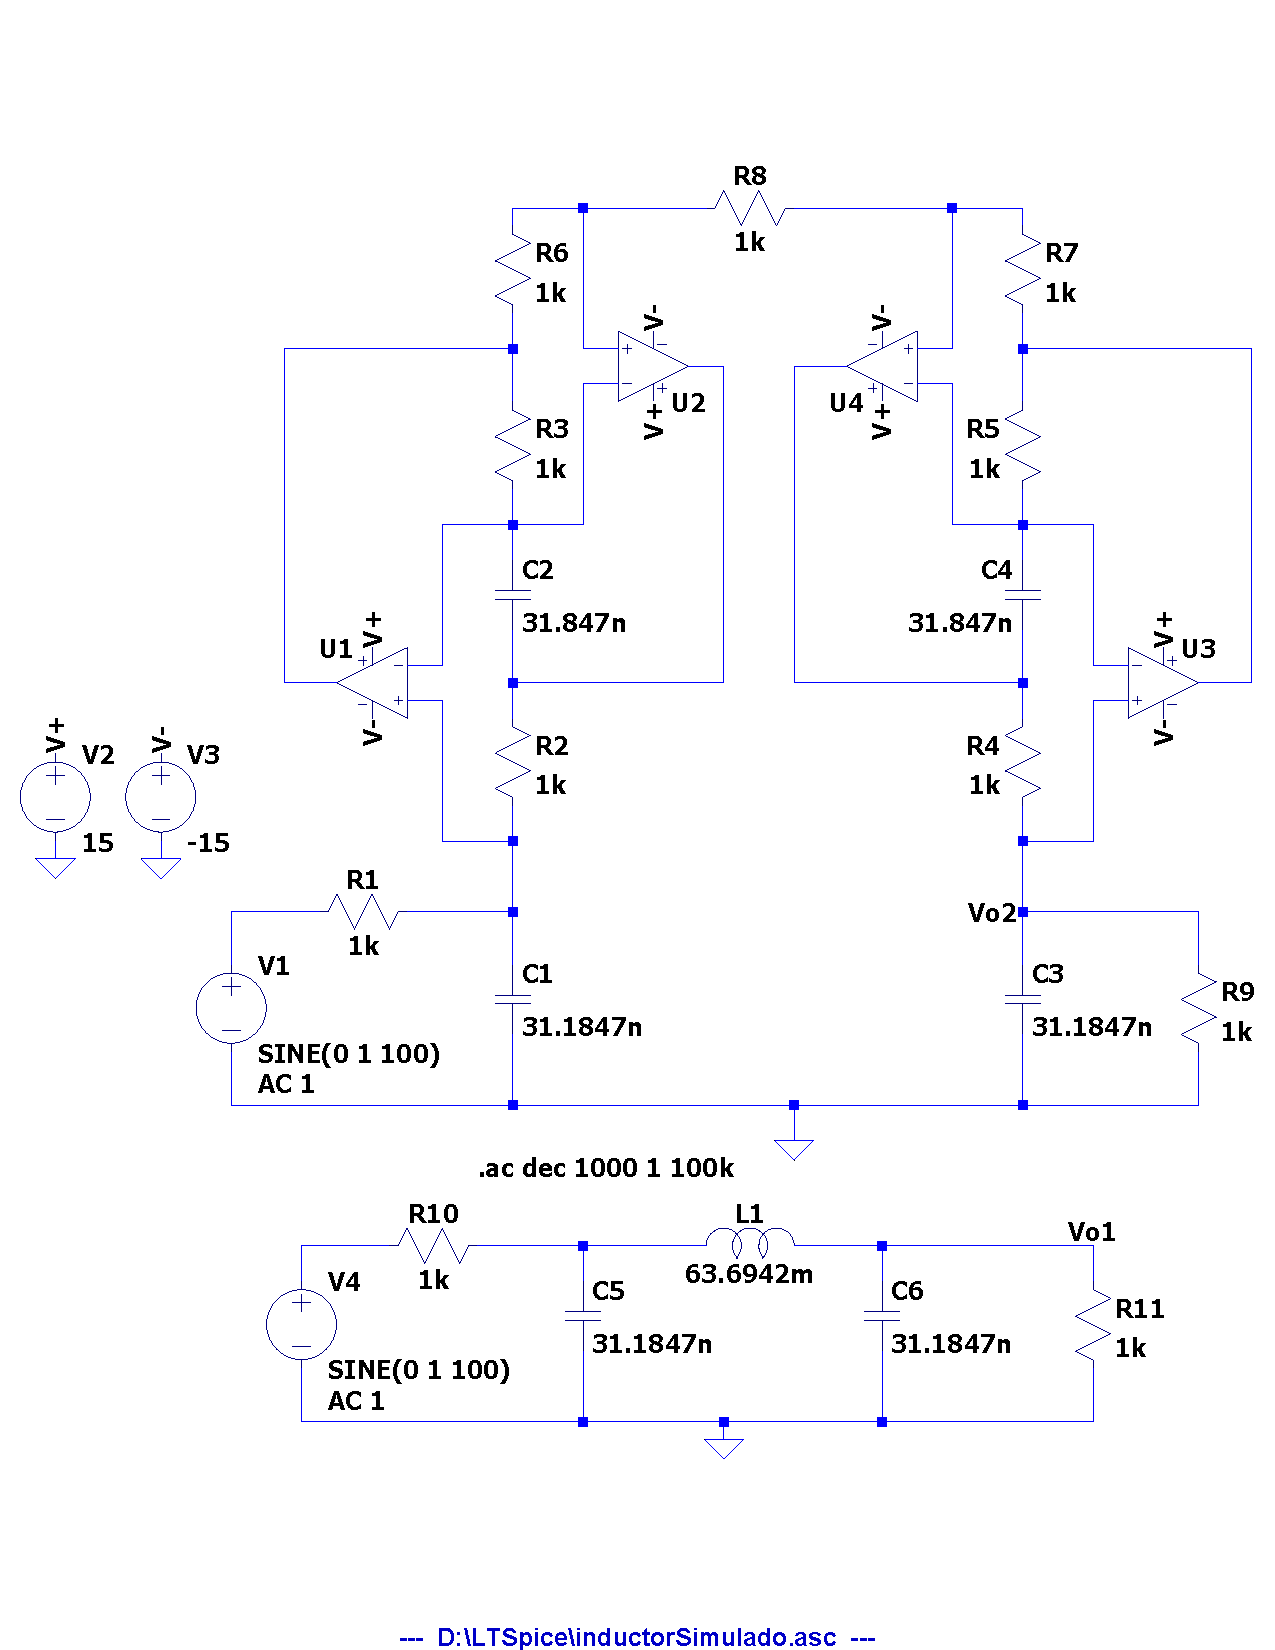
\includegraphics[clip, trim=0cm 3cm 0cm 2cm, width=\textwidth]{inductorSimulado1}
	\caption{Circuito esquemático}	
	\label{fig:figura10}
\end{figure}

\begin{figure}[H]
	\centering
	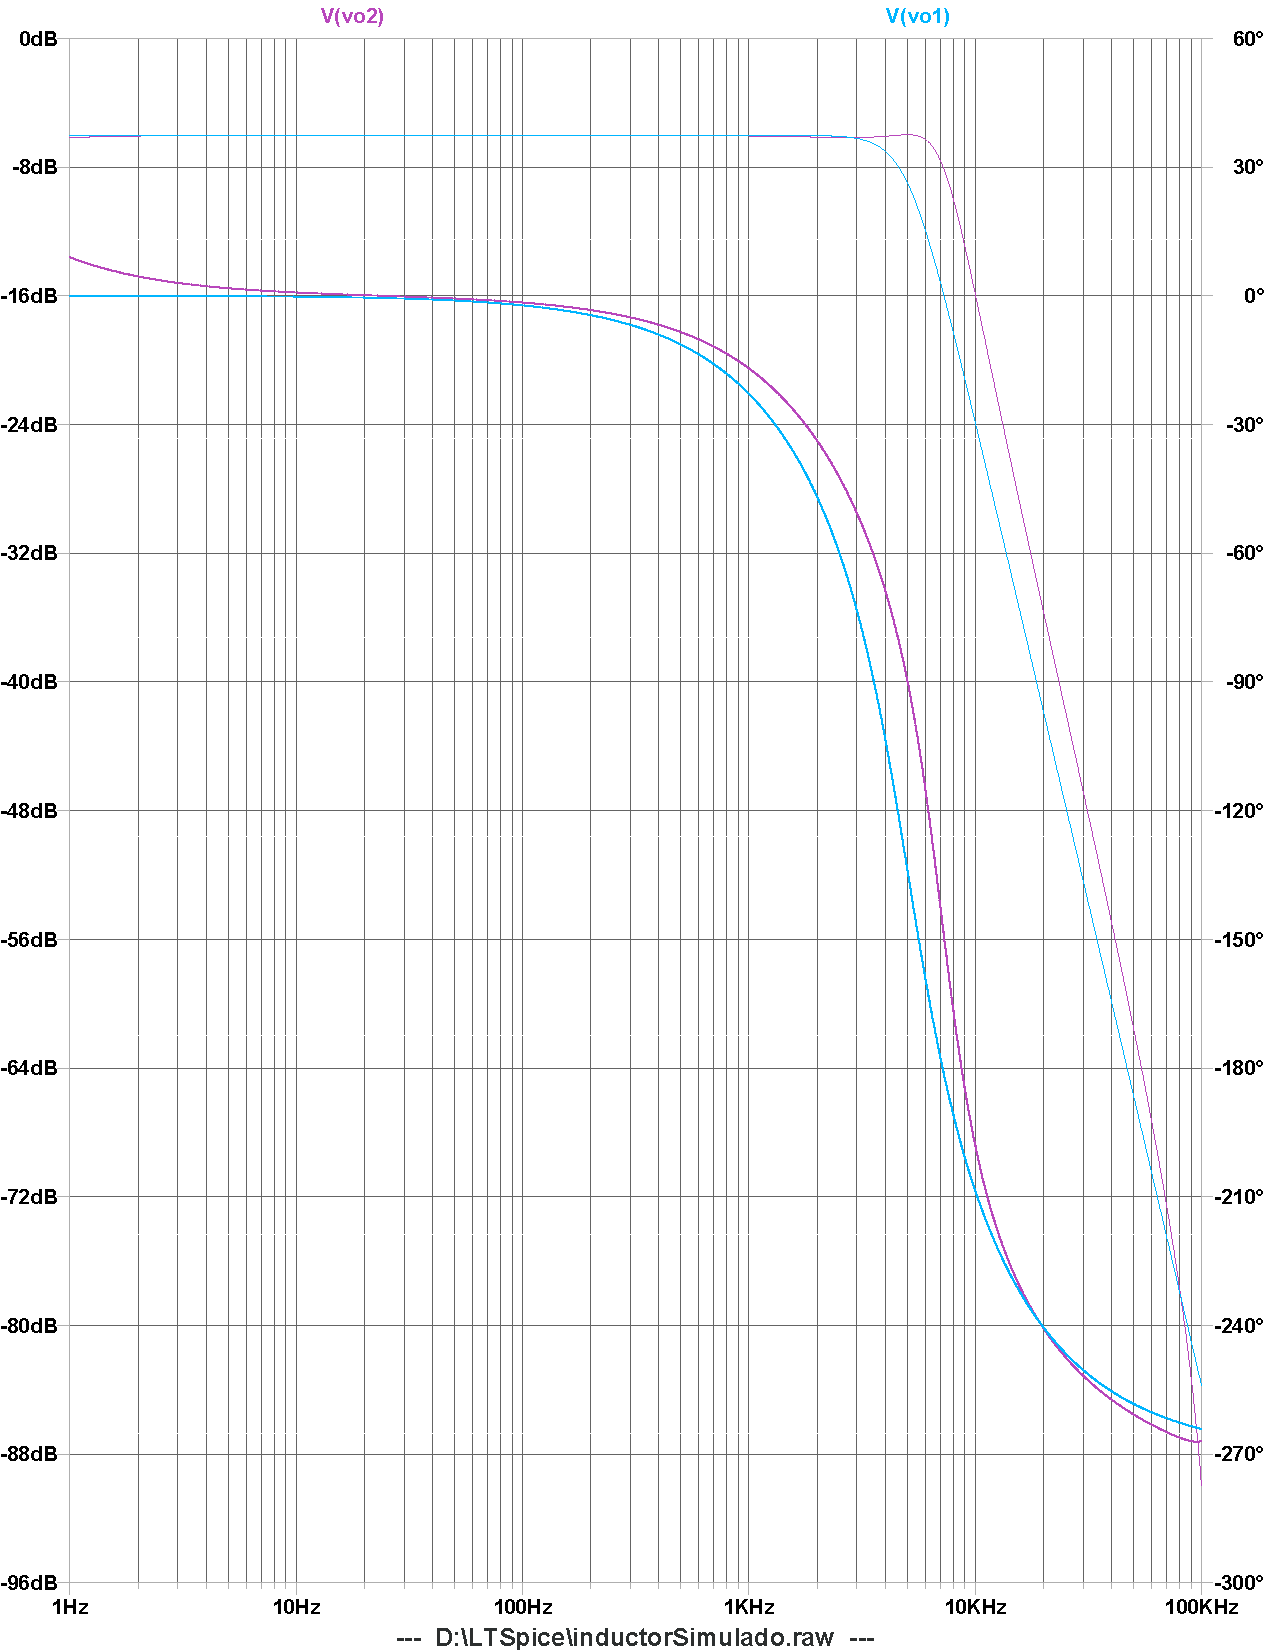
\includegraphics[clip, trim=0cm 0.5cm 0cm 0cm, width=\textwidth]{inductorSimuladoPlot1}
	\caption{Comparación de la respuesta en frecuencia}	
	\label{fig:figura11}
\end{figure}

\newpage
Ahora analizaremos el circuito de Riordan para simular un inductor flotante conectando circuitos de Riordan espalda con espalda como se muestra en la figura 11

	\begin{figure}[H]
	\centering	
	\begin{tikzpicture}[scale=0.8]
		%\ctikzset{resistor = european}
		\ctikzset{bipoles/thickness=4}
		\ctikzset{monopoles/vcc/arrow={Stealth[width=6pt,length=9pt]}}
		\ctikzset{monopoles/vee/arrow={Stealth[width=6pt,length=9pt]}}
		\draw (0,0) node[op amp, noinv input up, anchor=+](OA1){$OA_1$};
		\draw (OA1.-) to[short] ++(-1,0)
		to[short] ++(0,-2) coordinate (p1);
		\draw (p1) to[C, l=$C_2$] (p1 -| OA1.out) to[short] (OA1.out) node[above]{$V_1$};
		\draw (p1) to[R, *-, l=$R_1$] ++(0,-4) coordinate (z1);
		\draw (OA1.out) to[R, *-*, l=$R_3$] ++(4,0) node[above]{$V_n$} coordinate (p2);
		\draw (p2) to[short] ++(1,0) coordinate (p3);
		\draw (p3) node[op amp, noinv input up, anchor=-](OA2){$OA_2$};
		\draw (p2) to[short] ++(0,-2) coordinate (p4);
		\draw (p4) to[R, l=$R_4$] (p4 -| OA2.out) to[short] (OA2.out);
		\draw (OA2.+) to[short] ++(-1,0)
		to[short] ++(0,2) coordinate (p5) node[above]{$E_1(s)$};
		\draw (p5) to[R, l=$R_5$] (p5 -| OA2.out) to[short, -*] (OA2.out) coordinate (np) node[right]{$V_2$};		
		\draw (OA1.+) to[short] ++(-1,0) coordinate (p6) to[short] (p1|-p5) to[short, -*] (p5);
		\draw (p6) to[short, *-o, f_<=$I_1(s)$] ++(-2,0) coordinate (z2) node[left]{$E_1(s)$};
		\draw (z1) to[R, l=$R_1$] ++(0,-4) coordinate (c1);
		\draw (c1) to[short] ++(0,-2) -- ++(1,0) node[op amp, anchor=-](OA3){$OA_3$};
		\draw (c1) to[C, l=$C_2$, *-] (c1 -| OA3.out) to[short] (OA3.out);		
		\draw[->]  (z1)++(-0.5,0.2) node[left]{$$} -- ++(0,-1);
		\draw (OA3.out) node[below]{$V_3$} to[R, l=$R_3$, *-*] ++(4,0) coordinate (k1);
		\draw (k1) to[short] ++(1,0) node[op amp, anchor=-](OA4){$OA_4$};
		\draw (k1) to[short] ++(0,2) coordinate (k2);
		\draw (k2) to[R, l=$R_4$] (k2 -| OA4.out) to[short] (OA4.out) node[right]{$V_4$};
		\draw (OA4.+) to[short] ++(-1,0) to[short] ++(0,-2) node[below]{$E_2(s)$} coordinate (k3);
		\draw (k3) to[R, *-, l=$R_5$] (k3 -| OA4.out) to[short] (OA4.out);
		\draw (OA3.+) to[short] ++(-1,0) coordinate (k4);
		\draw (k3) -| (k4);
		\draw[-Triangle] (p6)++(3, 3) node[above right]{$I_1(s)$} -- ++(1,0) coordinate (f1);
		\draw (k4) to[short, *-o, f=$I_2(s)$] ++(-2,0) node[left]{$E_2(s)$};
	\end{tikzpicture}
	\caption{Inductor simulado de Riordan sustituyendo las impedancias por sus elementos resistivos y capacitivo}	
	\label{fig:figura12}
\end{figure}

\end{document}